\section{Background}\label{sec:background}

In this section we give an overview on Java bytecode, a brief
overview on dependence analysis, including control-flow and
data-flow testing criteria, and also a brief overview on program
slicing and on static metrics. In case of Java bytecode, the
interested reader can consult~\cite{Lindholm99JVMS} for a complete
reference about the JVM specification, as well as, the bytecode
instruction set. Considering dependence analysis on Java bytecode,
the interested reader can refer to~\cite{Zhao00DAJB}. More details
on control-flow and data-flow testing criteria can be found
in~\cite{Rapps85SSTD,Sinha99CTEH}. A good survey on program
slicing can be found in~\cite{Tip95SPST}. The static metrics
implemented in \toolname can be found
elsewhere~\cite{Lorenz94OOSM,Chidamber94MSOO}.

\subsection{Java Bytecode}\label{sec-bytecode}

One of the main reasons why Java has become so popular is the
platform independence provided by its runtime environment, the
Java Virtual Machine (JVM). The so called \emph{class} file is a
portable binary representation that contains class related data
such as the class name, its superclass name, information about the
variables and constants and the bytecode instructions of each
method.

Bytecode instructions can be seen as an assembly-like language
that retains high-level information about the program. A bytecode
instruction is represented by a one-byte opcode followed by
operand values, if any. Each one-byte opcode has a mnemonic that
is more meaningful than the opcode itself. The instructions are
typed and a letter preceding the mnemonic name represents the data
type handled by each instruction explicitly. The convention is to
use the letter \bci{i} for integer, \bci{l} for long, \bci{s} for
short, \bci{b} for byte, \bci{c} for char, \bci{f} for float,
\bci{d} for double, and \bci{a} for reference (objects and
arrays). For example, the instruction that pushes a one-byte
integer value onto the top of the JVM operand stack has the opcode
16, mnemonic \bci{bipush}, and requires one operand (the one-byte
integer value). The instruction \bci{bipush 9} pushes the value 9
onto the top of the JVM operand stack.

The JVM has a stack frame on which a frame is inserted for every
method invocation. Such a frame is composed by a local variable
vector, which contains all the local variables used in the current
method, and by an operand stack to perform the execution of the
bytecode instructions. For instance, considering the statement
``\mbox{\pk{a = b + c}}'', part of the local variable vector and
part of the operand stack required to execute such a statement are
illustrated in Figure~\ref{fig:jvm}.

\begin{figure}[!ht]\cmdsize
\begin{center}
\begin{tabular}{ll}
\begin{tabular}{|c|c|}\hline
\multicolumn{1}{|c|}{\textbf{Slot}}&\multicolumn{1}{|c|}{\textbf{Variable}}\\\hline
$\cdots$&$\cdots$\\\hline 2            & \var{a} \\\hline 3
& \var{b} \\\hline 4            & \var{c} \\\hline
$\cdots$&$\cdots$\\\hline
\multicolumn{2}{c}{(a) Local Variable Vector}\\
\end{tabular}
&
\begin{tabular}{|l|l|}\hline
\multicolumn{1}{|c|}{\textbf{Bytecode Instruction}} &
\multicolumn{1}{|c|}{\textbf{Operand Stack}} \\ \hline
12: iload\_3  & Value of \var{b} \\
              & $\cdots$         \\\hline
13: iload\_4  & Value of \var{c} \\
              & Value of \var{b} \\
              & $\cdots$         \\\hline
14: iadd      & Value of \var{b + c} \\
              & $\cdots$         \\\hline
15: istore\_2 & $\cdots$         \\\hline
\multicolumn{2}{c}{(b) Operand Stack Simulation}\\
\end{tabular}
\end{tabular}
\caption{Simple bytecode instruction execution.}\label{fig:jvm}
\end{center}
\end{figure}

Considering our example, variables \var{a}, \var{b} and \var{c}
correspond to local variables 2, 3 and 4, respectively. The
bytecode instructions \bci{iload\_3} and \bci{iload\_4} load the
value of \var{b} and \var{c} onto the top of the operand stack.
The instruction \bci{iadd} pops two operands from the stack,
executes the additions of such operands, and pushes back the
result onto the top of the stack. Finally, the instruction
\bci{istore\_2} pops the result from the top of the stack, storing
it into local variable 2 (variable \var{a}).

The complete set of bytecode instructions, illustrated in
Table~\ref{tab:bytecode} is composed by 204 instruction. From this
set, there are 3 reserved instructions and 43 that may raise an
exception (bytecode instructions highlighted in \textbf{bold}).
Only \bci{athrow} can throw an exception explicitly, all the
others 42 instructions may throw exceptions implicitly.

Although bytecode instructions resemble an assembly-like language,
a class file retains very high-level information about a program.
The idea behind \toolname is to provide as much information as
possible, such that the user can have a better understanding of
the program, even if the original source code is not available. In
the next section we explain how to collect control-flow and
data-flow information from the bytecode and how to use this
information to provide intra-method coverage criteria for Java
programs at bytecode level.

\subsection{Dependence Analysis for Java Bytecode}\label{sec:dependence}

The section below was extracted from~\cite{Vincenzi03JBSD} and is
replicated here with minor changes.

The most common underlying model to establish control-flow testing
criteria~\cite{McCabe76CMEA,Roper94STES} is the control-flow graph
(CFG), from which the testing requirements are derived. Data-flow
testing
criteria~\cite{Herman76DFAA,Rapps85SSTD,Maldonado91CPUC-EN} use
the Def-Use graph (\DUG), which is an extension of the CFG with
information about the set of variables defined and used in each
node and each edge of the CFG. In this report, the \DUG for Java
bytecode is called \emph{data-flow block graph} (\BG). From the
\BG both control and data-flow testing requirements can be
derived.


\begin{table}[!ht]
\begin{center}\scriptsize
\caption{Bytecode instruction set}\label{tab:bytecode}
\begin{tabular}{|p{1in}|p{2in}|p{2.75in}|}\hline
\textbf{Group}               & \textbf{Subgroup}                &   \textbf{Instruction Set}\cr\hline
Do nothing                   & -                                &   \bci{nop}\cr\hline
Load and Store               & Load a local variable
                               onto the operand stack           &   \bci{aload}, \bci{aload\_$\langle$n$\rangle^\dag$},
                                                                    \bci{dload}, \bci{dload\_$\langle$n$\rangle$},
                                                                    \bci{fload}, \bci{fload\_$\langle$n$\rangle$},
                                                                    \bci{iload}, \bci{iload\_$\langle$n$\rangle$},
                                                                    \bci{lload}, \bci{lload\_$\langle$n$\rangle$}\cr\cline{2-3}
                             & Store a value from the operand
                               stack into a local variable      &   \bci{astore}, \bci{astore\_$\langle$n$\rangle$},
                                                                    \bci{dstore}, \bci{dstore\_$\langle$n$\rangle$},
                                                                    \bci{fstore}, \bci{fstore\_$\langle$n$\rangle$},
                                                                    \bci{istore}, \bci{istore\_$\langle$n$\rangle$},
                                                                    \bci{lstore}, \bci{lstore\_$\langle$n$\rangle$}\cr\cline{2-3}
                             & Load a constant onto
                               the operand stack                &   \bci{bipush}, \bci{sipush},
                                                                    \bci{ldc}, \bci{ldc\_w},
                                                                    \bci{ldc2\_w}, \bci{aconst\_null},
                                                                    \bci{dconst\_$\langle$d$\rangle$}, \bci{fconst\_$\langle$f$\rangle$},
                                                                    \bci{iconst\_m1}, \bci{iconst\_$\langle$i$\rangle$},
                                                                    \bci{lconst\_$\langle$l$\rangle$}\cr\cline{2-3}
                             & Giving access to more
                               local variables using
                               a wider index or to a
                               larger immediate operand         &   \bci{wide}\cr\hline
Arithmetic                   & Add                              &   \bci{dadd}, \bci{fadd},
                                                                    \bci{iadd}, \bci{ladd}\cr\cline{2-3}
                             & Subtract                         &   \bci{dsub}, \bci{fsub},
                                                                    \bci{isub}, \bci{lsub}\cr\cline{2-3}
                             & Multiply                         &   \bci{dmul}, \bci{fmul},
                                                                    \bci{imul}, \bci{lmul}\cr\cline{2-3}
                             & Divide                           &   \bci{ddiv}, \bci{fdiv},
                                                                    \twb{idiv}, \twb{ldiv}\cr\cline{2-3}
                             & Remainder                        &   \bci{drem}, \bci{frem},
                                                                    \twb{irem}, \twb{lrem}\cr\cline{2-3}
                             & Negate                           &   \bci{dneg}, \bci{fneg},
                                                                    \bci{ineg}, \bci{lneg}\cr\cline{2-3}
                             & Shift                            &   \bci{ishl}, \bci{ishr},
                                                                    \bci{iushr}, \bci{lshl},
                                                                    \bci{lshr}, \bci{lushr}\cr\cline{2-3}
                             & Bitwise                          &   \bci{iand}, \bci{ior},
                                                                    \bci{ixor}, \bci{land},
                                                                    \bci{lor}, \bci{lxor}\cr\cline{2-3}
                             & Local Variable Increment         &   \bci{iinc}\cr\cline{2-3}
                             & Comparison                       &   \bci{dcmpg}, \bci{dcmpl},
                                                                    \bci{fcmpg}, \bci{fcmpl},
                                                                    \bci{lcmp}\cr\hline
Type Conversion              & -                                &   \bci{d2f}, \bci{d2i},
                                                                    \bci{d2l}, \bci{f2d},
                                                                    \bci{f2i}, \bci{f2l},
                                                                    \bci{i2b}, \bci{i2c},
                                                                    \bci{i2d}, \bci{i2f},
                                                                    \bci{i2l}, \bci{i2s},
                                                                    \bci{l2d}, \bci{l2f},
                                                                    \bci{l2i}\cr\hline
Object Creation              & Create Class Instance            &   \twb{new}\cr\cline{2-3}
and Manipulation             & Create Array                     &   \twb{newarray}, \twb{anewarray},
                                                                    \twb{multianewarray}\cr\cline{2-3}
                             & Access Fields of Classes         &   \twb{getfield}, \twb{getstatic},
                                                                    \twb{putfield}, \twb{putstatic}\cr\cline{2-3}
                             & Load an array component
                               onto the operand stack           &   \twb{aaload}, \twb{baload},
                                                                    \twb{caload}, \twb{daload},
                                                                    \twb{faload}, \twb{iaload},
                                                                    \twb{laload}, \twb{saload}\cr\cline{2-3}
                             & Store a value from the
                               operand stack as an
                               array component                  &   \twb{aastore}, \twb{bastore},
                                                                    \twb{castore}, \twb{dastore},
                                                                    \twb{fastore}, \twb{iastore},
                                                                    \twb{lastore}, \twb{sastore}\cr\cline{2-3}
                             & Get the array length             &   \twb{arraylength}\cr\cline{2-3}
                             & Check properties of
                               class instances or arrays        &   \twb{checkcast}, \twb{instanceof}\cr\hline

Control Transfer             & Unconditional Branch             &   \bci{goto}, \bci{goto\_w},
                                                                    \bci{jsr}, \bci{jsr\_w},
                                                                    \bci{ret}, \twb{athrow}\cr\cline{2-3}
                             & Conditional Branch               &   \bci{if\_acmpeq}, \bci{if\_acmpne},
                                                                    \bci{if\_icmpeq}, \bci{if\_icmpge},
                                                                    \bci{if\_icmpgt}, \bci{if\_icmple},
                                                                    \bci{if\_icmplt}, \bci{if\_icmpne},
                                                                    \bci{ifeq}, \bci{ifge},
                                                                    \bci{ifgt}, \bci{ifle},
                                                                    \bci{iflt}, \bci{ifne},
                                                                    \bci{ifnonnull}, \bci{ifnull}\cr\cline{2-3}
                             & Compound Conditional Branch      &   \bci{lookupswitch}, \bci{tableswitch}\cr\hline
Method Access                & Invocation                       &   \twb{invokeinterface}, \twb{invokespecial},
                                                                    \twb{invokestatic}, \twb{invokevirtual}\cr\cline{2-3}
                             & Return                           &   \twb{areturn}, \twb{dreturn},
                                                                    \twb{freturn}, \twb{ireturn},
                                                                    \twb{lreturn}, \twb{return}\cr\hline
Stack Management             & -                                &   \bci{dup}, \bci{dup\_x1},
                                                                    \bci{dup\_x2}, \bci{dup2},
                                                                    \bci{dup2\_x1}, \bci{dup2\_x2},
                                                                    \bci{pop}, \bci{pop2}, \bci{swap}\cr\hline
Synchronization              & -                                &
\twb{monitorenter}, \twb{monitorexit}\cr\hline Reserved
& -                                &   \bci{breakpoint},
\bci{impdep1}, \bci{impdep2}\cr\hline
\multicolumn{3}{l}{$^\dag\langle$n$\rangle$ represents a valid index
into the local variable array of the current frame~\cite{Lindholm99JVMS}.}\cr
\end{tabular}
\end{center}
\end{table}


Before constructing the \BG for a method, we construct its
\emph{data-flow instruction graph} (\IG). Informally, an \IG is a
graph where each node contains a single bytecode instruction and
the edges connect instructions that might be executed in sequence.
\IG also contains information about the kind of accesses
(definition or use) the bytecode instructions make. The \BG is
obtained by applying a reduction algorithm to the \IG. Such an
algorithm combines several \IG nodes in a single \BG node by
identifying blocks of bytecode instructions that are always
executed in sequence. The construction of \IG and \BG requires
static analysis of Java bytecode instructions. In
Sections~\ref{sec:icfg} and~\ref{sec:data-info} we explain how to
construct the \IG and how the data-flow information is collected,
respectively. In Section~\ref{sec:bcfg} the algorithm to generate
the \BG from the \IG is described.


\subsubsection{Constructing the Instruction Graph}\label{sec:icfg}

Some features of Java bytecode should be carefully handled when
performing control-flow analysis:

\begin{itemize}
    \item The use of intra-method subroutine calls. The JVM has two
    instructions \bci{jsr} and \bci{ret} that allow a piece of
    the method code to be ``called'' from several points in the
    same method. This is used to implement the \bci{finally}
    block of Java.

    \item Exception handlers. Each piece of code inserted in a
    \bci{catch} block in a Java program is an exception handler.
    The execution of such code is not done by ordinary control flow,
    but by the throwing of an exception.
\end{itemize}

To deal with the exception-handling mechanism of Java two kinds of
edges are used in the \IG: \textbf{primary edges} representing the
regular control-flow, \ie, when no exception is thrown; and
\textbf{secondary edges} representing the exception-handling
control-flow.

Formally, an \IG of a method $m$ is defined as a directed graph
$\mathcal{IG}(m) = (NI, EI_p, EI_s, si, TI)$ where each node $n
\in NI$ contains a single instruction of $m$. $EI_p$ represents
the set of primary edges and $EI_s$ the set of secondary edges. If
an instruction $j$, corresponding to the node $n_j \in NI$, can be
executed after an instruction $i$, corresponding to the node $n_i
\in NI$, then a primary edge from $n_i$ to $n_j$ exists,
$(n_i,n_j) \in EI_p$. If an instruction $i$, corresponding to the
node $n_i \in NI$, is in the scope of an exception-handler that
begins in an instruction $j$, corresponding to the node $n_j \in
NI$, then a secondary edge exists from $n_i$ to $n_j$, $(n_i,n_j)
\in EI_s$\footnote{In this way an exception-handler always
    begins a new node in the \IG or in the \BG since it
    is the target of one or more secondary edges.}.
The start node $si$ corresponds to the node that contains the
first instruction of $m$. Conversely, $TI$ is the set of
termination nodes, \ie, nodes that contain an instruction that
ends the method execution.

Consider the Java source code presented in
Figure~\ref{fig:average}(a). The class \pk{Vet} contains a method
\pk{Vet.average} that calculates and returns the average of an
array of integer numbers. The bytecode instructions that represent
the \pk{Vet.average} method are presented in
Figure~\ref{fig:average}(b). Each bytecode instruction is preceded
by a program counter number (\pc) that identifies a single
bytecode instruction inside a given method. In our example, the
first bytecode instruction \bci{aload\_0} is located at \pc 0 and
the last instruction (\bci{freturn}) at \pc 101.

Figure~\ref{fig:average}(c) illustrates the exception table for
\pk{Vet.average} method. The exception table indicates, for each
segment of bytecode instruction (\emph{from} and \emph{to}
columns), the beginning of the valid exception-handler
(\emph{target} column), and the corresponding type of exceptions
caught by such a handler (\emph{type} column). For example, from
\pc 12 to \pc 54 the valid exception-handler begins at \pc 60 and
it is responsible to catch any exception of the class
\pk{java.lang.Exception} or any one of its subclasses. A
registered exception handler with a $\langle$\textsf{Class
all}$\rangle$'s type catches any kind of exceptions.

\begin{figure}[!ht]
\begin{center}
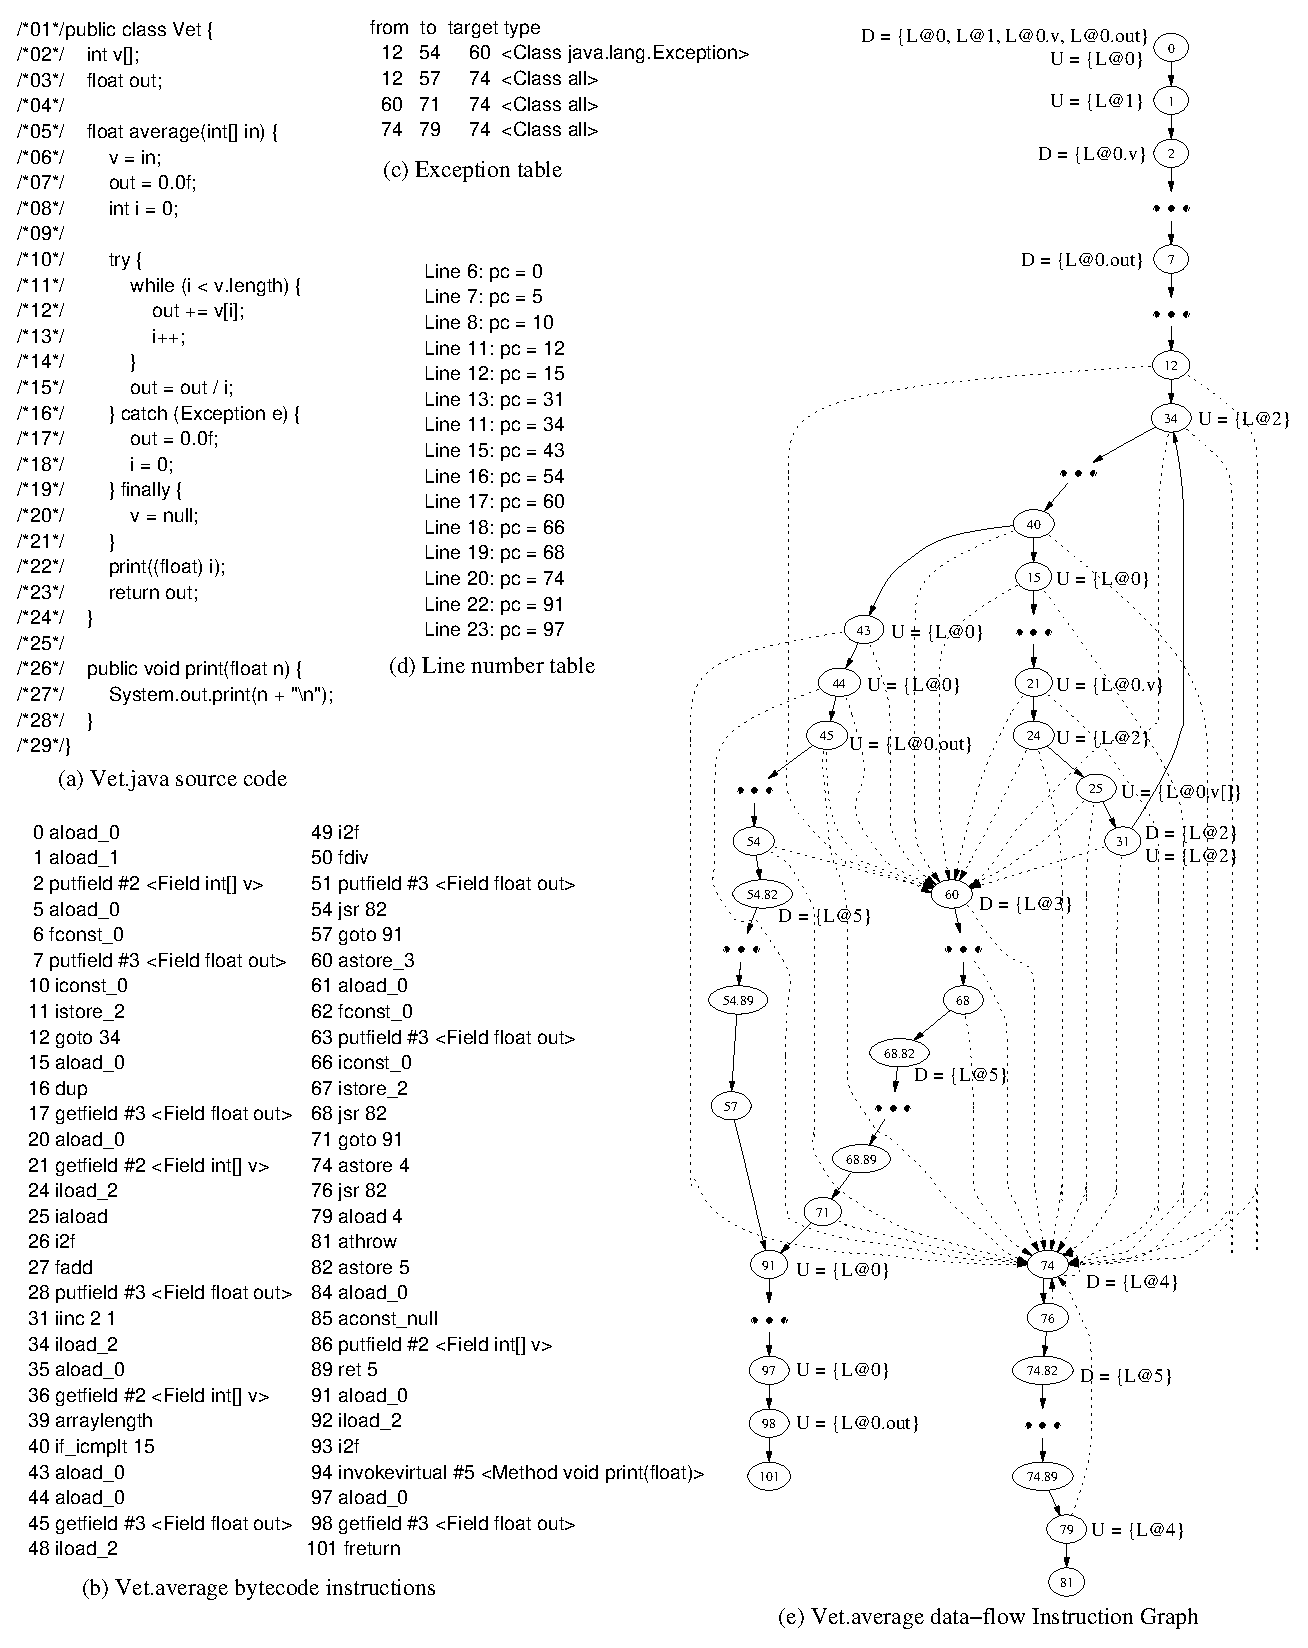
\includegraphics[width=0.9\textwidth]{fig/Vet.average.all.eps}
\caption{Illustration of the data-flow \IG.}\label{fig:average}
\end{center}
\end{figure}


The bytecode instructions can be related to source code lines
because the class file stores information that maps each bytecode
instruction to the source line it appears on. Thus, if the source
code is available, analysis applied on the bytecode level can be
mapped back to the source code level. The line number table,
illustrated in Figure~\ref{fig:average}(d), gives the
correspondence between source line number and bytecode program
counter. For example, the statement at the source line number 06
corresponds to the bytecode instructions from \pc 0 to \pc 2. The
bytecode instructions from \pc 5 to 7 correspond to the statement
at source line 07, and so on.

To construct \IG, the bytecode of a given method is read and an
interpreter is responsible for analyzing the semantics of each
instruction, identifying the set of nodes and edges of the \IG.
First, a node is created in the \IG for each bytecode instruction,
and such nodes are connected by primary edges, considering the
existence of control transfer between each instruction, and by
secondary edges, considering the exception table. From the
complete set of bytecode instructions presented in
Table~\ref{tab:classes} (Section~\ref{sec:data-info}), the
instructions in bold from Class~0 and Class~1 (first and second
rows) are related with the control-flow aspect of Java bytecode.
Figure~\ref{fig:average}(e) illustrates the resulting \IG of the
method presented in Figure~\ref{fig:average}(b). The \IG nodes are
numbered according to the \pc number of the bytecode instruction
it represents. Section~\ref{sec:data-info} describes how to
identify the set \var{D$_i$} of defined variables and the set
\var{U$_i$} of used variables associated to each node of \IG.
Observe that at bytecode level it is not possible to distinguish
between a \emph{p-use} and a \emph{c-use}. Later, in the
computation of the data-flow criteria, nodes with more than one
outgoing edge will have the uses associated to such edges, as if
they were \emph{p-uses}.

Since in the \IG each bytecode instruction corresponds to a node,
the number of nodes and edges can be very large, even for methods
with a few lines of code. In case of the \IG in
Figure~\ref{fig:average}(e), some nodes are omitted in order to
reduce the size of the \IG and to make it more readable. Ellipsis
(``$\bullet \bullet \bullet$'') are used to represent omitted
nodes.

Primary edges are represented by continuous lines and secondary
edges by dotted lines. Observe that there are a large number of
secondary edges connecting the nodes in the scope of a given
exception-handler to the first node of the handler. For example,
according to the exception table of Figure~\ref{fig:average}(c)
the exception-handler located at \pc 60 is responsible to catch
all exceptions of \pk{java.lang.Exception} class raised from \pc
12 to \pc 54. So, there are secondary edges connecting all nodes
in this range to node 60. The same applies to the other
exception-handlers.

Special care on building the \IG is required to deal with
subroutine calls inside the method, used, for example, to
implement the \bci{finally} block of Java. Each \bci{jsr}
instruction causes the execution of an intra-method piece of code
(subroutine). After the subroutine has been executed, the
execution is resumed at a different point in the program,
depending on which \bci{jsr} caused the execution of the
subroutine. In our example, there are three \bci{jsr} instructions
located at \pc 54, 68, and 76, all of them representing a branch
to \pc 82, that is the first instruction of the \bci{finally}
block. Such a finally block goes from \pc 82 to \pc 89. Observe
that at \pc 89 there is a \bci{ret} instruction which returns the
execution to \pc 57, 71 or 79, depending on which \bci{jsr}
instruction invoked the subroutine. To avoid any misinterpretation
about which \bci{jsr} instruction causes the invocation of the
\bci{finally} block, and at which instruction the execution is
resumed, the set of nodes that corresponds to the \bci{finally}
block is replicated for each \bci{jsr} instruction, and different
labels are used to identify the replicated nodes. In our example,
nodes 82 to 89 are replicated three times and the labels of such
nodes are preceded by ``54.'', ``68.'', and ``76.'', as can be
observed in Figure~\ref{fig:average}(e).
Figure~\ref{fig-single-finally} illustrates the problem if the
nodes that compose a \bci{finally} block are not replicated.
Observe that since node 82 has three incoming edges and node 89
three outgoing edges this can lead to the false impression that
from any incoming edge there are three outgoing edges while, in
the reality, only one exists. By replicating the nodes in the
subroutine we avoid such a problem, as illustrated in
Figure~\ref{fig-multiple-finally}.

\begin{figure}[!ht]
\begin{center}
\subfigure[]{\label{fig-single-finally}\includegraphics[scale=0.30]{fig/single-finally.eps}}\qquad\qquad\qquad
\subfigure[]{\label{fig-multiple-finally}\includegraphics[scale=0.30]{fig/multiple-finally.eps}}
\caption{Different approaches to deal with \bci{finally} block:
(a) Single Finally Node (b) Multiple Finally
Nodes.}\label{fig-finally}
\end{center}
\end{figure}


\subsubsection{Augmenting the \IG: Data-Flow
\IG}\label{sec:data-info}

The first thing required to augment the \IG with data-flow
information is to precisely define the underlying data-flow model
which indicates what kinds of bytecode instructions lead to
variable definition/use and also how to consider reference and
array variables. By analyzing the set of bytecode instructions
obtained from~\cite{Lindholm99JVMS} we classify such instructions
in eleven different classes, according to their relation with the
data-flow at bytecode level. Table~\ref{tab:classes} illustrates
these classes of instructions.

\begin{table}[!ht]
\caption{Different classes of bytecode
instruction.}\label{tab:classes}
\begin{center}\scriptsize
\begin{tabular}{|c|p{0.4\textwidth}|p{0.4\textwidth}|}\hline
\textbf{Class}&\textbf{Bytecode Instructions}&\textbf{Data-Flow Implication}\\\hline
0   & \setbci{\ctrl{athrow}, \ctrl{goto}, \ctrl{goto\_w},
    \ctrl{if\_acmpeq}, \ctrl{if\_acmpne}, \ctrl{if\_icmpeq}, \ctrl{if\_icmpge},
    \ctrl{if\_icmpgt}, \ctrl{if\_icmple}, \ctrl{if\_icmplt}, \ctrl{if\_icmpne},
    \ctrl{ifeq}, \ctrl{ifge}, \ctrl{ifgt}, \ctrl{ifle}, \ctrl{iflt}, \ctrl{ifne},
    \ctrl{ifnonnull}, \ctrl{ifnull}, \ctrl{lookupswitch}, \ctrl{tableswitch},
    \ctrl{areturn}, \ctrl{dreturn}, \ctrl{freturn}, \ctrl{ireturn}, \ctrl{lreturn}, \ctrl{return},
    \ctrl{ret},
    monitorenter, monitorexit, pop, pop2,
    breakpoint, impdep1, impdep2, nop,
    checkcast,
    wide, swap} &
    Instructions in this class have \textbf{no implication} for the flow of data.\\\hline
1   &  \setbci{\ctrl{invokeinterface}, \ctrl{invokespecial}, \ctrl{invokestatic}, \ctrl{invokevirtual},
    \ctrl{jsr}, \ctrl{jsr\_w},
    dadd, ddiv, dmul, dneg, drem, dsub, fadd, fdiv, fmul, fneg, frem, fsub,
    iadd, iand, idiv, imul, ineg, ior, irem, ishl, ishr, isub, iushr, ixor,
    ladd, land, ldiv, lmul, lneg, lor, lrem, lshl, lshr, lsub, lushr,
    lxor,
    arraylength, instanceof,
    aconst\_null, bipush, dconst, fconst, iconst, lconst, sipush,
    ldc, ldc\_w, ldc2\_w,
    d2f, d2i, d2l, f2d, f2i, f2l, i2b, i2c, i2d, i2f, i2l, i2s, l2d, l2f,
    l2i,
    new, multianewarray, anewarray, newarray,
    dcmpg, dcmpl, fcmpg, fcmpl, lcmp}
    &
    Instructions in this class have \textbf{no implication} for the flow of data.
    In addition, they leave an unknown element at the top of the operand stack.
    Accesses to such element will not characterize any use or definition. For example,
    instruction \bci{new} pushes an object reference onto the stack. Further use
    of such reference as a field access is not regarded as a definition or use.\\\hline
2   & \setbci{aaload, baload, caload, daload, faload,
    iaload, laload, saload}
    & Loads an array element to the top of the operand stacks and
    indicating the \textbf{use} of the array.\\\hline
3   & \setbci{aastore, bastore, castore, dastore,
    fastore, iastore, lastore, sastore}
    & Stores the value on the top of the operand stack
    into an array element, indicating the \textbf{definition} of the array.\\\hline
4   & \setbci{putfield}
    & Stores the value on the top of the operand stack into an
    instance field, indicating the \textbf{definition} of such an instance field.\\\hline
5   & \setbci{putstatic}
    & Stores the value on the top of the operand stack into a
    class field, indicating the \textbf{definition} of such a class field.\\\hline
6   & \setbci{dup, dup2, dup\_x1, dup\_x2, dup2\_x1, dup2\_x2}
    & Duplicates the value onto the top of the operand stack and
    has \textbf{no implication} for the flow of data.\\\hline
7   & \setbci{aload, dload, fload, iload, lload}
    & Loads the value of a given local variable onto the top
    of the operand stack, indicating a \textbf{use} of such a local variable.\\\hline
8   & \setbci{astore, dstore, fstore, istore, lstore}
    & Stores the value on
    the top of the operand stack into a local variable,
    indicating a \textbf{definition} of such a variable.\\\hline
9   & \setbci{getfield}
    & Loads an instance field onto the top of the operand stack,
    indicating a \textbf{use} of such an instance field.\\\hline
10  & \setbci{getstatic}
    & Loads a class field onto the top of the operand stack,
    indicating a \textbf{use} of such a class field.\\\hline
11  & \setbci{iinc}
    & Increments the value of a given local variable,
    indicating a \textbf{use} and a
    \textbf{definition} of such a local variable.\\\hline
\end{tabular}
\end{center}
\end{table}


The division into such classes was based on the kind of
definitions and uses that we would like to identify. In Java and
Java bytecode, the variables can be classified in two types: basic
or reference types. Fields of a class can be of basic or reference
type and are classified as instance or class fields, depending on
whether they are unique to each object of the class or unique to
the entire class (static fields), respectively. Local variables
declared inside a method can also be of basic or reference type.
An aggregated variable (array) is of reference type. To deal with
aggregated variables we are following the approach proposed by
Horgan and London~\cite{Horgan91DFCC}, which considers an
aggregated variable as a unique storage location such that when a
definition (use) of any element of the aggregated variable occurs,
what is considered to be defined (used) is the aggregated variable
and not a particular element. Moreover, in their data-flow model,
a definition of a given variable blocks previous definitions of
the same variable. So, in our data-flow model the following
guidelines apply to identify definitions and uses of variables:

\begin{enumerate}
    \item Aggregated variables are considered as a unique
    storage location and the definition/use of any element of
    the aggregated variable \var{a[]} is considered to be a
    definition/use of \var{a[]}. So, in the statement
    ``\var{a[i] = a[j] + 1}'' there is a definition and a use of
    the aggregated variable \var{a[]}.

    \item If an aggregate variable \var{a[][]} is defined, an access to
    its elements is considered a definition or use of \var{a[][]}. Then,
    in the statement ``\var{a[0][0] = 10}'' there exists a definition
    of \var{a[][]} and in the statement ``\var{a[0] = new
    int[10]}'' there is a definition of \var{a[]}.

    \item Every time an instance field (or an array element)
    is used (defined) there is a use of the reference variable used to access the field
    and a use (definition) of the field itself. Considering
    \var{ref\_1} and \var{ref\_2} as reference variables of a class
    \var{C} which contains two instance fields \var{x} and \var{y} of
    type \var{int}, in the statement ``\var{ref\_1.x = ref\_2.y}''
    there are uses of the reference variables \var{ref\_1} and \var{ref\_2},
    a use of the instance field \var{ref\_2.y}, and a definition of the
    instance field \var{ref\_1.x}. Since instance fields are valid in
    the entire scope of a given class, each instance field
    used in the context of a given method is considered
    to have a definition in the first node of the \IG.

    \item Class fields (static fields) can be considered as global variables
     and do not require a reference variable to be
     accessed. Considering a class \var{C} with
     a static fields \var{w} and \var{z}, in the statement
     ``\var{C.z = C.w + y}'' there are a use of \var{C.w} and a definition of
     \var{C.z}. Even if a static field is accessed using a
     reference variable \var{ref\_1} of class \var{C}, such that
     ``\var{ref\_1.w = 10}'', at bytecode level, such a reference is
     converted to the class name and there is no use of the
     reference variable in this statement. Since
     static fields are in the entire scope of a given class,
     each static field used in the context of a given method is
     considered to have a definition in the first node of the \IG.

    \item A method invocation such as \var{ref\_1.foo(e\_1, e\_2, $\ldots$, e\_n)} indicates
    a use of the reference variable, \var{ref\_1}. The rules for
    definition and use identification inside expressions \var{\mbox{e\_1, e\_2, $\ldots$,
    e\_n}} are the same as described on items 1 to 4.

    \item For instance methods, a definition of \bci{this} is assigned to the
    first node of the \IG, and also the definition of each local variable
    corresponding to the formal parameters of such a method, if any.
    For class methods, only the local variables corresponding to the parameters
    are considered, no instance is required to invoke such a method.
\end{enumerate}

Based on these guidelines and on the different classes of bytecode
instructions, the \IG of a given method is traversed and to each
node of such a graph a set \var{D$_i$} of defined variables, and a
set \var{U$_i$} of used variables are assigned. Before explaining
how these two sets are created, it is important to know how these
different kinds of variables are treated at the bytecode level.
Method parameters and variables declared inside the method are
treated as local variables and are bound to the JVM local variable
table as follows: if it is an instance method, local variable
zero, referenced here as \var{L@0}, is bound to the reference to
the current object (\var{this}), \ie, the object that caused the
method invocation. The formal parameters, if any, are bound to the
local variable one (\var{L@1}), two (\var{L@2}), and so on,
depending on the type and on the number of parameters. Finally,
the variables declared inside the method are bound to the
remaining local variables, also depending on the type and the
number of declared variables. For example, considering the source
code of the method \pk{Vet.average}, it can be observed that it is
an instance method which accepts one parameter \var{in} and
declares one local variable \var{i}. \var{L@0} corresponds to
reference to the current object. The formal parameter \var{in}
corresponds to \var{L@1}, and the variable \var{i} corresponds to
\var{L@2}. Three other local variables (\var{L@3}, \var{L@4} and
\var{L@5}) are used by the compiler to implement the
exception-handling mechanism. The method accesses two instance
fields: \var{v}, and \var{out}. Since they are instance fields,
they require a reference to an object of class \pk{Vet} to be
accessed. When no reference is used preceding a field, the
reference to the current object is used. So, \var{v} and \var{out}
are referenced in the bytecode of our example as \var{L@0.v} and
\var{L@0.out}.

To analyze the \IG we implemented a simulator that interprets
bytecode instructions and identifies the type and the source of
data manipulated by each instruction. For example, suppose the
current instruction to be analyzed is \bci{iload\_2}. Such an
instruction, when interpreted by the JVM, pushes onto the top of
the operand stack an integer value stored in \var{L@2}. Our
simulator, instead of pushing an actual value, pushes onto the top
of the stack an indication in the form ``\pk{$<$type$>$ -
$<$data\_source$>$}'' to be used when interpreting the next
bytecode instructions. \pk{$<$type$>$} corresponds to the data
type being manipulated, and \pk{$<$data\_source$>$} to the source
of each data. In this example, instruction \bci{iload\_2} pushes
an indication like ``\pk{int - L@2}'', since \var{L@2} is a data
source of an integer value. Moreover, the load instruction
characterizes a use of \var{L@2} so this variable is inserted in
the set of used variables associated to the current node of the
\IG graph. Different indications are used to represent the
different types of storage places, as described above. In
Figure~\ref{diff-conf}(a), second column, there are different
kinds of indications placed onto the top of the operand stack when
the bytecode instructions in the first column are interpreted. For
a class field (static field) the indication is in the form
``\pk{$<$type$>$ - S@$<$class\_name$>$.$<$field\_name$>$}'', where
\pk{$<$type$>$} is the type of the static field,
\pk{$<$class\_name$>$} is the class name, and
\pk{$<$field\_name$>$} is the name of the static field. A detailed
description of the interpreter and all kinds of indications can be
found in~\cite{Vincenzi03STOO}.

Considering the \IG presented in Figure~\ref{fig:average}(e),
there are the definitions of \var{L@0}, \var{L@1}, \var{L@0.v},
and \var{L@0.out} associated with node~0. Moreover, node~0 also
contains a bytecode instruction of Class~7 (\bci{aload\_0}), which
indicates a use of the loaded local variable, \var{L@0} in this
case. Observe that the bytecode instruction at \pc 0 is one of the
bytecode instructions that corresponds to the statement ``\var{v =
in}'' at source code line 6 of Figure~\ref{fig:average}(a). The
use exists because before initializing such a field, which is
carried out when the instruction located at \pc 2 is executed, the
reference to the current object (\var{L@0}) has to be loaded onto
the top of the operand stack, characterizing the use of such a
local variable.

At node~2, the \bci{putfield} instruction, which belongs to
Class~4, indicates a definition of an instance field, in our case
the instance field \var{v}, referenced as \var{L@0.v}. So, the set
of defined variables at node~2 contains the element \var{L@0.v}.
Finally, the instruction at node~25, \bci{iaload}, belongs to
Class~2 and indicates a use of an element of an array of integers,
so the set of used variables at node~25 contains the element
\var{L@0.v[]}.

One important point to be observed is that, when evaluating a
given instruction, the current top of the operand stacks can have
more that one configuration, depending on the path used to reach
the instruction. Since it is possible to reach a given node
through different instruction sequences, each different possible
stack configuration needs to be evaluated to find the complete set
of defined/used variables in a \IG node. This is performed by
traversing the \IG as many times as necessary, until all possible
combinations have been evaluated, and the complete set of
defined/used variables on each node have been found.

As an example of such a situation, consider the bytecode
instructions illustrated in Figure~\ref{diff-conf}(b). This set of
bytecode instructions corresponds to the piece of source code
shown in Figure~\ref{diff-conf}(a). Figure~\ref{diff-conf}(c)
shows the corresponding data-flow \IG.

Observe that the bytecode instruction at node~30, can be reached
from two different paths: \{16, 17, 20, 23, 24, 28, 30\} or \{16,
17, 20, 27, 28, 30\}. Each of them inserts a different indication
in the top of the operand stack, the first loads \var{L@1} into
the top of the operand stack and the other \var{L@2}. When
executing the bytecode instruction at \pc 30, which stores the
value onto the top of the operand stack in a field of an object,
two possible combinations can occur, the definition of the field
\var{x} of \var{L@1}, or the definition of field \var{x} of
\var{L@2}. Therefore, the complete set of defined variables at \IG
node 30 contains both: \var{L@1.x} and \var{L@2.x}.

\begin{figure}[!ht]
\begin{center}\scriptsize
\begin{tabular}{cc}
\begin{minipage}{0.50\textwidth}
\hspace{1cm}
\begin{tabular}{|l|l|}\hline
\multicolumn{2}{|l|}{\var{r = new Foo();}}\\
\multicolumn{2}{|l|}{\var{s = new Foo();}}\\
\multicolumn{2}{|l|}{\var{(r.x == 0 ? r : s).x = 20;}}\\\hline
\multicolumn{2}{c}{(a) Piece of Java Source Code}\\
\multicolumn{2}{c}{}\\
\multicolumn{2}{c}{}\\\hline \textbf{Bytecode
Instruction}&\textbf{Operand Stack Configuration}\\ \hline \bci{16
aload\_1}        & \begin{minipage}{0.3\textwidth}
                               Foo - L@1\\
                               $\cdots$
                         \end{minipage}\\ \hline
\bci{17 getfield \#4 $<$Field int x$>$}&
\begin{minipage}{0.3\textwidth}
                               int - L@1.x\\
                               $\cdots$
                         \end{minipage}\\ \hline
\bci{20 ifne 27}        & \begin{minipage}{0.3\textwidth}
                               $\cdots$
                         \end{minipage}\\ \hline
\bci{23 aload\_1}        & \begin{minipage}{0.3\textwidth}
                               Foo - L@1\\
                               $\cdots$
                         \end{minipage}\\ \hline
\bci{24 goto 28}        & \begin{minipage}{0.3\textwidth}
                               Foo - L@1\\
                               $\cdots$
                         \end{minipage}\\ \hline
\bci{27 aload\_2}        & \begin{minipage}{0.3\textwidth}
                               Foo - L@2\\
                               $\cdots$
                         \end{minipage}\\ \hline
\bci{28 bipush 20}        & \begin{minipage}{0.3\textwidth}
                               int - DC\\
                               \textbf{Foo - L@1 or Foo - L@2}\\
                               $\cdots$
                         \end{minipage}\\ \hline
\bci{30 putfield \#4 $<$Field int x$>$}&
\begin{minipage}{0.3\textwidth}
                               \textbf{int - L@1.x or int - L@2.x}\\
                               $\cdots$
                         \end{minipage}\\ \hline
\end{tabular}
\end{minipage}
&
\begin{minipage}{0.50\textwidth}
\hspace{3cm}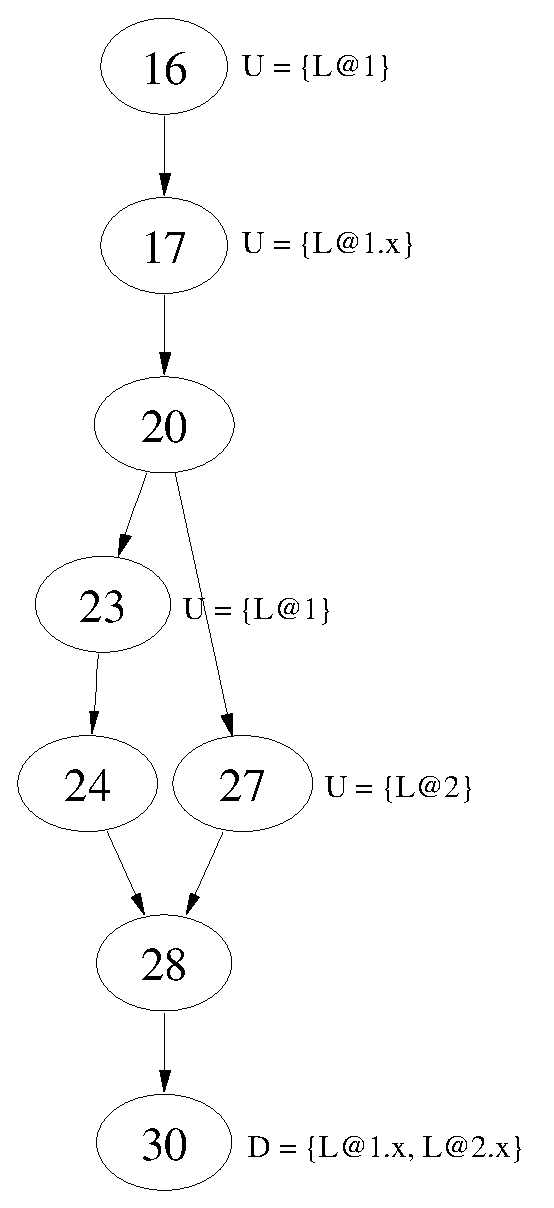
\includegraphics[width=0.38\textwidth]{fig/diff-conf.eps}
\end{minipage}\\
\multicolumn{1}{c}{\hspace{2cm}(b) Bytecode instructions}&
\multicolumn{1}{c}{(c) Corresponding \IG}\\
\end{tabular}
\end{center}
\caption{Different Stack Configurations.}\label{diff-conf}
\end{figure}

Once the complete set of defined and used variables have been
detected, the instruction CFG can be reduced to originate the \BG.
The algorithm used to perform such a reduction is explained in the
next section.

\subsubsection{Constructing Data-Flow Block Graph
(\BG)}\label{sec:bcfg}

The \IG provides a practical way to traverse the set of statements
of a given method to identify the set of variables defined and
used by each statement. However, since a node on \IG is created
for each statement of a given method $m$, the number of nodes and
edges can be very large, especially considering lower level
bytecode instructions. Once all information about each bytecode
instruction has been collected, we use the concept of
\emph{instruction block} to reduce the number of nodes and edges
as much as possible.

An \emph{instruction block} is a set of instructions that are
``normally'' executed in sequence in a program. When the first
instruction of a block is executed, so are the remaining
instructions; branching only occurs to the beginning and from the
end of the block.

A block graph for a given method $m$ is a directed graph
$\mathcal{BG}(m) = (N, E_p, E_s, s, T)$ such that, each node $n
\in N$ represents a instruction block, each edge $(n_i, n_j) \in
E_p$ represents a primary edge (control transfer) between blocks
$n_i$ and $n_j$, each edge $(n_i, n_j) \in E_s$ represents a
secondary edge between blocks $n_i$ and $n_j$, $s$ corresponds to
the start block, and $T$ is the set of termination blocks. For
each block two sets \var{D$_i$} and \var{U$_i$} are assigned. They
contain the sets of defined and used variables in the block,
respectively.

The algorithm used to reduce a data-flow \IG to a data-flow  \BG
is presented in Figure~\ref{fig:algorithm}. In line 14 of the
algorithm, a decision is taken whether the current instruction $x$
being analyzed is the last one in the current block or not. It
will be the last one if at least one of the following conditions
holds:

\begin{itemize}
   \item $x$ is a jump, goto, ret or invoke instruction;
   \item $x$ has more than one primary successor;
   \item the single primary successor of $x$ has more than
         one (primary or secondary) predecessor;
   \item the single primary successor of $x$ has not the
         same set of secondary successors of $x$.
\end{itemize}

\begin{figure}[!ht]
{\cmdsize
\begin{center}
\begin{tabular}{|l|}\hline\\
\begin{minipage}{5in}
\noindent\# Input: $iG$, the instruction-CFG $GI = \langle NI, EI_p,EI_s, si, TI\rangle$ to be reduced; \\
\# Output: $bG$, the block CFG $bG = \langle N, E_p, E_s, s,
T\rangle$
\\ \ \\
%
01\bigind    s := NewNodeTo(si) \\
02\bigind    foreach $x \in N$ \\
03\bigind    \ind if $x$ has no successor \\
04\bigind    \ind\ind $T := T \cup \{x\}$ \\ \ \\
%
     \# Auxiliary function: NewNodeTo \\
     \# Input: A node $y$ from $iG$ \\
     \# Output: A node from $bG$ where $y$ has been inserted \\ \ \\
%
05\bigind     $ins$ := the instruction in $y$ \\
06\bigind     if the node $y$ has already been visited \\
07\bigind     \ind return the node $w \in N$ that contains $ins$ \\
08\bigind     $CurrentNode :=$ new block node \\
09\bigind     $N := N \cup \{CurrentNode\}$ \\
10\bigind     $x := y$ \\
11\bigind     repeat \\
12\bigind     \ind Include $x$ as part of $CurrentNode$ \\
13\bigind     \ind Mark $x$ as visited \\
14\bigind     \ind if $x$ should terminated the current block \\ % aqui � linha xx
15\bigind     \ind\ind foreach $v$ such that $(x,v) \in EI_p$ \\
16\bigind     \ind\ind\ind $E_p := E_p \cup \{(CurrentNode, NewNodeTo(v))\}$ \\
17\bigind     \ind\ind foreach $v$ such that $(x,v) \in EI_s$ \\
18\bigind     \ind\ind\ind $E_s := E_s \cup \{(CurrentNode, NewNodeTo(v))\}$ \\
19\bigind     \ind\ind $x := null$ \\
20\bigind     \ind else \\
21\bigind     \ind\ind if there exists a $v$ such that $(x,v) \in EI_p$ \\
22\bigind     \ind\ind\ind $x := v$ \\
23\bigind     \ind\ind else \\
24\bigind     \ind\ind\ind $x := null$ \\
25\bigind     while $x \neq null$ \\
26\bigind     return $CurrentNode$ \\
\end{minipage}\\\hline
\end{tabular}
\end{center}
}
\caption{Algorithm to generate the CFG from bytecode.}\label{fig:algorithm}
\end{figure}


Zhao~\cite{Zhao99ACFJ} proposes a different approach to construct
the CFG of a given method. According to Zhao's approach, if an
exception-handler is present, a new node is also created for any
instruction that may throw an exception explicitly (instruction
\bci{athrow}) or implicitly (other 42 instructions), which can
increase significantly the number of nodes in the CFG. Moreover,
to correctly implement the approach to generate the CFG as
proposed by Zhao~\cite{Zhao99ACFJ} it is necessary to check the
subclasses of each exception that may be raised and to identify if
there is any exception-handler that can catch this particular
exception. In our implementation we decide to use a more pragmatic
approach to construct the \BG, expecting to obtain simpler and
more readable graphs.

As mentioned earlier, two points that should be highlighted are:
first, when we have subroutine calls, the set of statement blocks
representing the subroutine is expanded for every call, \ie, the
statements of a given subroutine may appear more than once in the
\BG within different nodes, once for each subroutine call.

Second, observe that since the set of bytecode instructions on
each statement block might not throw all kind of handled
exceptions, our \BG may have ``false'' (or spurious) secondary
edges. Moreover, the execution of a given block can be interrupted
in any place, when an exception is thrown, so in the presence of
exceptions the block may not have the ``atomicity'' characteristic
mentioned above. On the other hand, this approach simplifies both
the construction of the \BG and also its interpretation, since the
number of nodes is reduced. An alternative approach to construct a
CFG to deal with exception-handling constructions is described by
Sinha and Harrold~\cite{Sinha98APEH} such that no false edges are
generated. Although, the proposed technique considers only
exceptions generated explicitly, \ie, the ones originate by the
\bci{throw} statement~\cite{Sinha98APEH}.

%--------------------------------
%----
%----
%---- There is a good example and figure describing the
%---- exception-handling mechanism in the paper
%---- "Analysis of Programs with Exception-Handling Constructs"
%---- \cite{Sinha98APEH}
%----
%----
%--------------------------------

\begin{figure}[!ht]
\begin{center}
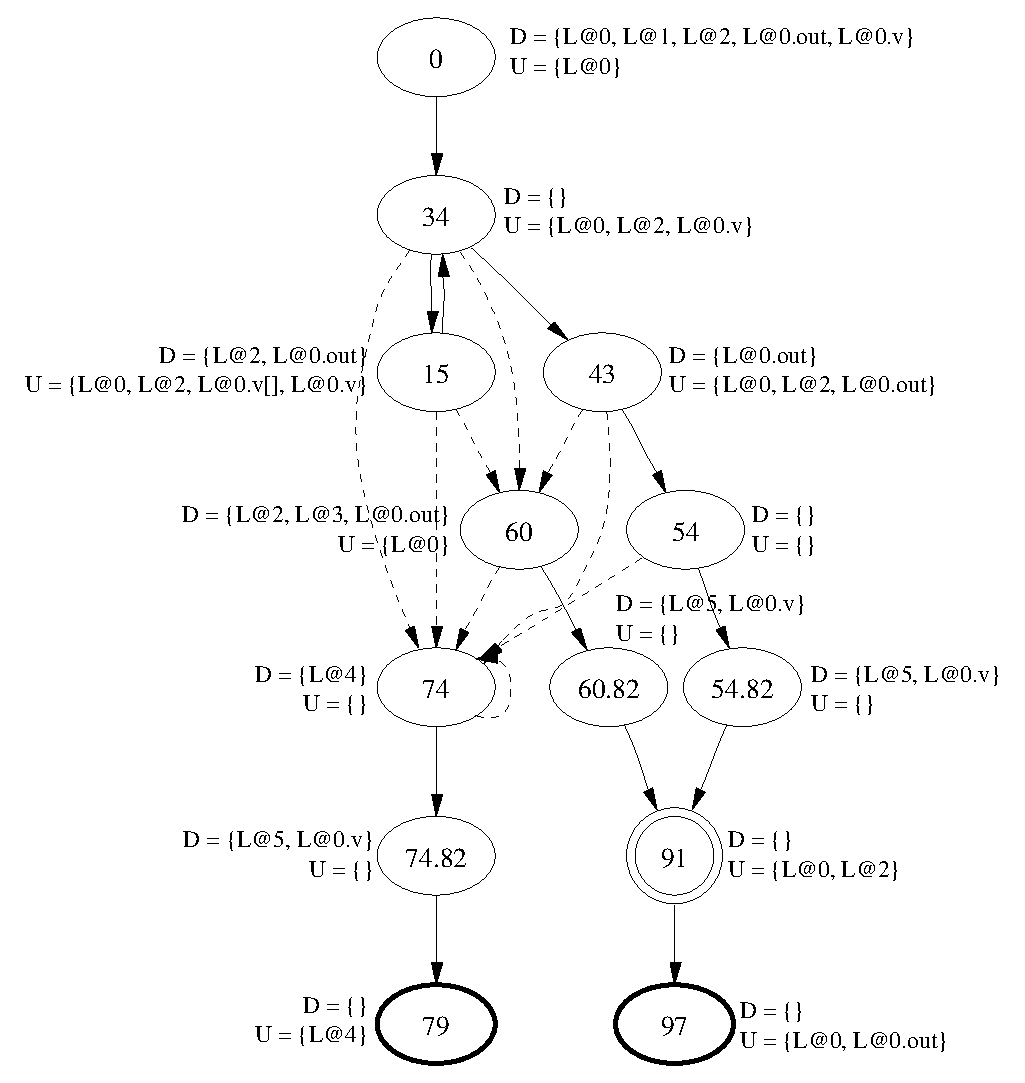
\includegraphics[scale=0.50]{fig/average-bcfg.eps}
\caption{\pk{Vet.average}'s \BG.}\label{fig-average-bcfg}
\end{center}
\end{figure}


After the \BG has been constructed, a simple analysis is carried
out to eliminate unnecessary nodes, \ie, nodes that contain only a
single \bci{goto} instruction. They can be eliminated by directly
connecting its in-coming edges as the in-coming edges of its
successor. Figure~\ref{fig-average-bcfg} illustrated the \BG
obtained by applying the reduction algorithm to the \IG of
Figure~\ref{fig:average}(e). \BG represents the underlying model
used to derive control-flow and data-flow testing requirements.
The label of a given block in \BG is the program counter number of
its first instruction. The labels of the replicated nodes, \ie,
nodes corresponding to a subroutine, are preceded by the label of
the node that invoked the subroutine. Observe that since
instruction node 68 of \IG now composes the block node 60 in \BG,
instructions nodes 68.82 of \IG correspond to block node 60.82 in
\BG. All the other replicated instruction nodes that correspond to
the finally block, \ie, instruction nodes 84, 85, 86 and 89 in
\IG, are part of the block nodes $xx$.82 in \BG.

On constructing the \BG we also have two different types of edges
to represent primary edges (continuous line) and secondary edges
(dashed lines). Moreover, we make a distinction among three
different types of nodes in \BG: termination nodes represented by
bold line circles (as blocks 79 and 97 in
Figure~\ref{fig-average-bcfg}); call nodes represented by double
line circles (as block 91 in Figure~\ref{fig-average-bcfg}); and
regular nodes represented by single line circles (as all other
nodes in Figure~\ref{fig-average-bcfg}). The call nodes are being
distinguished from the others because we intend to extend our
analysis to inter-method level; thus, call nodes are useful for
constructing the inter-method control-flow and data-flow graphs.
Def-use information is trivially computed for each \BG node by the
union of the definition (use) sets of each \IG node included in
the \BG node.

Once the \BG has been obtained, different testing criteria can be
applied to derive different testing requirements that can be used
to assess the quality of a given test set or to generate a given
test set. In the next section we describe some of the testing
criteria that we are working on and the set of testing
requirements derived from each one.

\subsection{Intra-method Structural Testing Requirements}\label{sec:criteria}

Java bytecode can be thought of as an assembly-like language from
that control-flow and data-flow information can be collected and
represented as a \BG, as described above. Once collected, such
information for each method, intra-method testing criteria can be
defined and applied. Basically, at method level, as mentioned
in~\cite{Harrold94PDFT}, traditional control-flow and data-flow
testing criteria~\cite{Rapps85SSTD} can be applied, since they are
based on the same underlying representation, \ie, the \BG. Sinha
and Harrold~\cite{Sinha99CTEH} describe a set of data-flow based
testing criteria considering exceptions. Thus we can adopt
coverage criteria for the later~\cite{Rapps85SSTD,Sinha99CTEH}. We
propose to conduct coverage testing on Java programs, including
Java components with respect to six different testing criteria:
four are control-flow-based and two are data-flow-based.

\subsubsection{Control-Flow Testing
Requirements}\label{sec:ctrl-requirements}

The \BG is a representation of a given method in a program.
Control-flow testing criteria can be derived based on such a
program representation to provide a theoretical and systematical
mechanism to select and assess the quality of a given test set. We
are using two well known control-flow testing criteria to derive
testing requirements from the \BG: \emph{all-nodes} and
\emph{all-edges}~\cite{Roper94STES}.

\begin{itemize}
    \item \textbf{all-nodes criterion}: requires that each \BG node has been
    exercised at least once by a test case in the test set. This criterion
    ensures that every statement in the method have been executed
    at least once by a given test case. we decided
    to subdivide such criterion in two non-overlapping testing
    criteria such that the tester can concentrate on different
    aspects of a program at a time:

    \begin{itemize}
        \item \textbf{all-primary-nodes}: requires that each primary
        node has been exercised at least once by a test case in the
        test set. This criterion requires that all statements not related
        with exception-handling mechanism were executed at least once;

        \item \textbf{all-secondary-nodes}: requires that each
        secondary node has been exercised at least once by a test case in the
        test set. This criterion requires that all statements related
        with exception-handling mechanism were executed at least once;
    \end{itemize}


    \item \textbf{all-edges criterion}: requires that each \BG edge
    has been exercised at least once by a test case in the test set.
    This criterion ensures that every possible control transfer in
    the method
    has been executed at least once by a given test case. Since
    in our \BG there are two different types of edges, we decided
    to subdivide such criterion in two non-overlapping testing
    criteria:

    \begin{itemize}
        \item \textbf{all-primary-edges}: requires that each primary
        edge has been exercised at least once by a test case in the
        test set. This criterion requires that all conditional
        expressions were evaluated as true and false at least once;

        \item \textbf{all-secondary-edges}: requires that each
        secondary edge
        has been exercised at least once by a test case
        in the test set. This criterion requires that each
        exception-handler be executed at least once from each node
        where an exception might be raised.
    \end{itemize}
\end{itemize}

To illustrate how such criteria can be applied,
Table~\ref{tab-ctrl-requirements} presents the set of testing
requirements required by each one of them, considering the \BG of
the method \pk{Vet.average} (Figure~\ref{fig-average-bcfg}).

\begin{table}[!ht]
\begin{center}\cmdsize
\caption{Set of control-flow testing requirements for
\pk{Vet.average} \BG.}\label{tab-ctrl-requirements}
\begin{tabular}{|c|c|p{0.6\textwidth}|}
  \hline
  % after \\: \hline or \cline{col1-col2} \cline{col3-col4} ...
  \multicolumn{2}{|c|}{\textbf{Criterion}} & \textbf{Testing Requirements} \\
  \hline
  \multirow{2}{1.5cm}{\centering all-nodes} &
    \multirow{1}{3cm}{\centering all-primary-nodes} & \{0, 15, 34, 43, 54, 54.82, 91, 97\} \\ \cline{2-3}
  & \multirow{1}{3cm}{\centering all-secondary-nodes} & \{60, 60.82, 74, 74.82, 79\} \\
  \hline

  \multirow{4}{1.5cm}{\centering all-edges} & \multirow{2}{3cm}{\centering all-primary-edges} & \{(0,34), (15,34), (34,15), (34,43), (43,54),
                                                         (54,54.82), (54.82,91), (60,60.82),
                                                         (60.82,91), (74,74.82), (74.82,79), (91,97) \} \\
               \cline{2-3}
  & \multirow{2}{3cm}{\centering all-secondary-edges} & \{(15,60), (15,74), (34,60), (34,74), (43,60), (43,74), (54,74),
  (60,74), (74,74)\} \\
  \hline
\end{tabular}
\end{center}
\end{table}

\subsubsection{Complexity Analysis of Control-Flow Testing
Criteria}

\rev{TO BE DONE...}

\subsubsection{Data-Flow Testing
Requirements}\label{sec:data-requirements}

With respect to data-flow testing, we are using the well known
\emph{all-uses} criterion~\cite{Rapps85SSTD} that is composed of
the \emph{all-c-uses} and \emph{all-p-uses} criteria. A precise
definition about these criteria can be found
in~\cite{Rapps85SSTD}. A {\em use} represents the use of a
variable in a statement. If the value of a variable is used for
some computation, it is a {\em c-use} (Computational Use), whereas
if the value is used in a predicate that determines which branch
is to be executed, it is a {\em p-use} (Predicate Use). Let $b_i$
and $b_j$ to be two points in the bytecode where a variable $x$ is
defined and used, respectively. This definition and this use are
referred to as $d_i(x)$ and $u_j(x)$, respectively. The pair
$(d_i(x), u_j(x))$ is a def-use pair if there is a definition
clear path with respect to $x$ from $b_i$ to $b_j$, \ie, $x$ is
not defined at any point other than $b_i$. The pair is also said
feasible if there exists a test case $t$ such that the execution
of the method on $t$ causes such definition clear path from $b_i$
to $b_j$ to be traversed.

For an example of a c-use, consider the \DUG of
Figure~\ref{fig-average-bcfg}. At node 0, the variable definition
set contains the variable \var{L@0.v}, which represents the
instance variable \var{v} in the corresponding source code. At
node 15 there is a use of \var{L@0.v} to compute the sum of its
elements, determining a c-use pair \wrt \var{L@0.v} from node 0 to
node 15 (c-use). On the other hand, at node 15, there is a
definition of \var{L@2} that represents the local variable \var{i}
in the corresponding source code. Such a variable is used in the
predicate located at node 34 to evaluate if the end of \var{v} has
been reached. Thus, there is a p-use pair \wrt \var{L@2} from node
15 to node 34. From the bytecode, it is not possible to
distinguish p-uses and c-uses. In our implementation of all-uses
criterion we assume that a use in a node with more than one
out-going edge is a p-use and associate it with each of those
edges. As with the all-edges criterion, we divided the all-uses
criterion such that two sets of non-overlapping testing
requirements are obtained, to consider the primary and secondary
edges. We named such criteria all-primary-uses and
all-secondary-uses, respectively. The first takes all the def-use
pairs for which there exists a path of primary edges only. The
other def-use pairs are required by the second.

To illustrate how such criteria can be applied,
Table~\ref{tab-data-requirements} presents the set of testing
requirements required by each one of than, considering the \BG of
the method \pk{Vet.average} (Figure~\ref{fig-average-bcfg}).

A test set $T$ may be evaluated against the all-uses criterion
(all-primary-uses/all-secondary-uses) by computing the ratio of
the number of def-use pairs covered to the total of all-uses
(all-primary-uses/all-secondary-uses) requirements. The same
applies to all-nodes and all-edges
(all-primary-edges/all-secondary-edges) criteria. More details
about the testing criteria definition can be found
in~\cite{Vincenzi03STOO}.

\begin{table}[!ht]
\begin{center}\cmdsize
\caption{Set of data-flow testing requirements for
\pk{Vet.average} \BG.}\label{tab-data-requirements}
\begin{tabular}{|c|c|ccc|}
  \hline
  % after \\: \hline or \cline{col1-col2} \cline{col3-col4} ...
  \multicolumn{2}{|c|}{\textbf{Criterion}} & \multicolumn{3}{l|}{\textbf{Testing Requirements}} \\
  \hline
  \multirow{20}{1.5cm}{\centering all-uses} & \multirow{10}{3cm}{\centering all-primary-uses} &
\ass{L@0}{0}{\edg{15}{34}} & \ass{L@0}{0}{\edg{34}{15}} &
\ass{L@0}{0}{\edg{34}{43}} \\ & & \ass{L@0}{0}{\edg{43}{54}} &
\ass{L@0}{0}{\edg{60}{60.82}} & \ass{L@0}{0}{54.82} \\ & &
\ass{L@0}{0}{60.82} & \ass{L@0}{0}{74.82} & \ass{L@0}{0}{91} \\ &
& \ass{L@0}{0}{97} & \ass{L@0.out}{0}{\edg{43}{54}} &
\ass{L@0.out}{15}{\edg{43}{54}} \\ & & \ass{L@0.out}{43}{97} &
\ass{L@0.out}{60}{97} & \ass{L@0.v}{0}{\edg{15}{34}} \\ & &
\ass{L@0.v}{0}{\edg{34}{15}} & \ass{L@0.v}{0}{\edg{34}{43}} &
\ass{L@0.v[]}{0}{\edg{15}{34}} \\ & & \ass{L@2}{0}{\edg{15}{34}} &
\ass{L@2}{0}{\edg{34}{15}} & \ass{L@2}{0}{\edg{34}{43}} \\ & &
\ass{L@2}{0}{\edg{43}{54}} & \ass{L@2}{0}{91} &
\ass{L@2}{15}{\edg{15}{34}} \\ & & \ass{L@2}{15}{\edg{34}{15}} &
\ass{L@2}{15}{\edg{34}{43}} & \ass{L@2}{15}{\edg{43}{54}} \\ & &
\ass{L@2}{15}{91} & \ass{L@2}{60}{91} & \ass{L@4}{74}{79}
\\\cline{2-5}
  & \multirow{11}{3cm}{\centering all-secondary-uses} &
\ass{L@0}{0}{\edg{15}{60}} & \ass{L@0}{0}{\edg{15}{74}} &
\ass{L@0}{0}{\edg{34}{60}} \\ & & \ass{L@0}{0}{\edg{34}{74}} &
\ass{L@0}{0}{\edg{43}{60}} & \ass{L@0}{0}{\edg{43}{74}} \\ & &
\ass{L@0}{0}{\edg{60}{74}} & \ass{L@0.out}{0}{\edg{43}{60}} &
\ass{L@0.out}{0}{\edg{43}{74}} \\ & &
\ass{L@0.out}{15}{\edg{43}{60}} & \ass{L@0.out}{15}{\edg{43}{74}}
& \ass{L@0.out}{43}{\edg{43}{60}} \\ & &
\ass{L@0.out}{43}{\edg{43}{74}} & \ass{L@0.v}{0}{\edg{15}{60}} &
\ass{L@0.v}{0}{\edg{15}{74}} \\ & & \ass{L@0.v}{0}{\edg{34}{60}} &
\ass{L@0.v}{0}{\edg{34}{74}} & \ass{L@0.v[]}{0}{\edg{15}{60}} \\ &
& \ass{L@0.v[]}{0}{\edg{15}{74}} & \ass{L@2}{0}{\edg{15}{60}} &
\ass{L@2}{0}{\edg{15}{74}} \\ & & \ass{L@2}{0}{\edg{34}{60}} &
\ass{L@2}{0}{\edg{34}{74}} & \ass{L@2}{0}{\edg{43}{60}} \\ & &
\ass{L@2}{0}{\edg{43}{74}} & \ass{L@2}{15}{\edg{15}{60}} &
\ass{L@2}{15}{\edg{15}{74}} \\ & & \ass{L@2}{15}{\edg{34}{60}} &
\ass{L@2}{15}{\edg{34}{74}} & \ass{L@2}{15}{\edg{43}{60}} \\ & &
\ass{L@2}{15}{\edg{43}{74}} & & \\\hline
\end{tabular}
\end{center}
\end{table}

\subsubsection{Complexity Analysis of Data-Flow Testing Criteria}

\rev{TO BE DONE...}

\subsection{Dominators and Super-Block Analysis}\label{sec:super-block}

Studies have shown that it is important to generate a test set
with high coverage while testing C programs so that more faults
are likely to be
detected\cite{Piwowarski93CMED,Wong94ETSS,Wong98ETSM}. The same
applies to Java programs without lost of generality. To explain
our approach to increase the coverage as soon as possible \wrt a
given test criterion (all-blocks in our example), consider the \BG
presented in Figure~\ref{fig-average-bcfg}. The main idea is to
assign different weights to each \BG node based on dominator
analysis and ``super block''~\cite{Agrawal94DSBP}. The objective
is to generate a test to cover one of the areas with the highest
weight, if possible, before other areas with a lower weight are
covered so that the maximum coverage can be added in each single
execution. In this way, we provide useful hints on how to generate
efficient test cases to increase, as much as possible with as few
tests as possible, the control-flow (such as block and decision)
and data-flow coverage (such as all-uses) of the programs being
tested.

Basically, a super-block is a subset of nodes with the property
that if any node in a super block is covered then all nodes in
that super block are covered\footnote{Assuming that the
    underlying hardware does not fail and no exception
    is raised during the execution of a test}. Pre- and
post-dominator relationships among nodes are used to identify the
set of super blocks from a given \BG. According
to~\cite{Agrawal94DSBP}, a node $u$ pre-dominates a node $v$
denoted as $u \stackrel{pre}{\rightarrow} v$, if every path from
the entry node to $v$ contains $u$. A node $w$ post-dominates a
node $v$ denoted as $u \stackrel{post}{\rightarrow} v$, if every
path from $v$ to the exit node contains $w$. For example, in
Figure~\ref{fig-average-bcfg}, nodes 0 and 34 pre-dominate node 74
and nodes 74.82 and 79 post-dominate it. Pre- and post-dominator
relationships can be expressed in the form of pre- and post
dominator trees, respectively. $u \stackrel{pre}{\rightarrow} v$
\emph{iff} there is a path from $u$ to $v$ in the predominator
tree. Similarly, $w \stackrel{post}{\rightarrow} v$ \emph{iff}
there is a path from $w$ to $v$ in the post-dominator tree.
Figures~\ref{fig-pre-dominator} and~\ref{fig-post-dominator} show
the pre- and post-dominator trees of the \BG in
Figure~\ref{fig-average-bcfg}.

The dominator relationship amongst \BG's nodes is represented by a
``basic block dominator graph'' that corresponds to the union of
the pre- and post-dominator trees. Figure~\ref{fig-merged-tree}
shows the basic block dominator graph of the \BG in
Figure~\ref{fig-average-bcfg}.

From the basic block dominator graph, strongly connected
components (super blocks) are identified and the corresponding
super block dominator graph is obtained. A strongly connected
component has a property that every node in the component
dominates all other nodes in that component. For example, nodes
\{74, 74.82, 79\} compose a strongly connected component.

Figure~\ref{fig-super-block} represents the super block dominator
tree of the \BG in Figure~\ref{fig-average-bcfg}. From this
representation it is possible to calculate the weight of each \BG
node. Basically, the weight of a given node is the number of nodes
that have not been covered but will be if that block is covered.
In Figure~\ref{fig-super-block-uncovered}, the initial weight of
each super block is show on the bottom of each node.

For example, to arrive at node 54.82 in
Figure~\ref{fig-average-bcfg} requires the execution also to go
through nodes 0, 34, 43, and 54. After arriving in node 54.82,
nodes 91 and 97 will also be executed. This implies node 54.82 is
dominated by nodes 0, 34, 43, 54, 91 and 97. It also means nodes
0, 34, 43, 54, 91 and 97 will be covered (if they haven't been) by
a test execution if that execution covers node 54.82. Assuming
none of the blocks is covered so far, we say that node 54.82 has a
weight of at least 7 because covering it will increase the
coverage by at least seven nodes. Using the same approach, node 15
has a weight of 3 since its coverage only guarantees an increase
of coverage by at least three nodes. A very important note is that
while assigning the weight to a given node, we use a conservative
approach by counting only the additional nodes that will
definitely be covered because of the coverage of this given node.
This is why we use the phrase ``at least'' in the above
statements. Of course, covering a node of a weight 7 (like node
54.82 in our example) may end up covering more than seven blocks
(por ex., the execution can go through nodes 0, 34, 15, 34, 43, 54
before it reaches node 54.82 and continues though nodes 91 and
97). Nevertheless, the additional nodes (node 15 in our example)
are not guaranteed to be covered.

\begin{figure}[!ht]
\begin{center}
\subfigure[Pre-Dominator
Tree]{\label{fig-pre-dominator}\includegraphics[scale=0.50]{fig/average-dominator-tree.eps}}\qquad
\subfigure[Post-dominator
Tree]{\label{fig-post-dominator}\includegraphics[scale=0.50]{fig/average-idominator-tree.eps}}

\subfigure[Basic Block Dominator
Tree]{\label{fig-merged-tree}\includegraphics[scale=0.50]{fig/average-merged-tree.eps}}\qquad
\subfigure[Super Block Dominator
Tree]{\label{fig-super-block}\includegraphics[scale=0.50]{fig/average-super-block.eps}}
\caption{Control-Flow Dependence Analysis.}\label{fig-super}
\end{center}
\end{figure}


\begin{figure}[!ht]
\begin{center}
\subfigure[]{\label{fig-super-block-uncovered}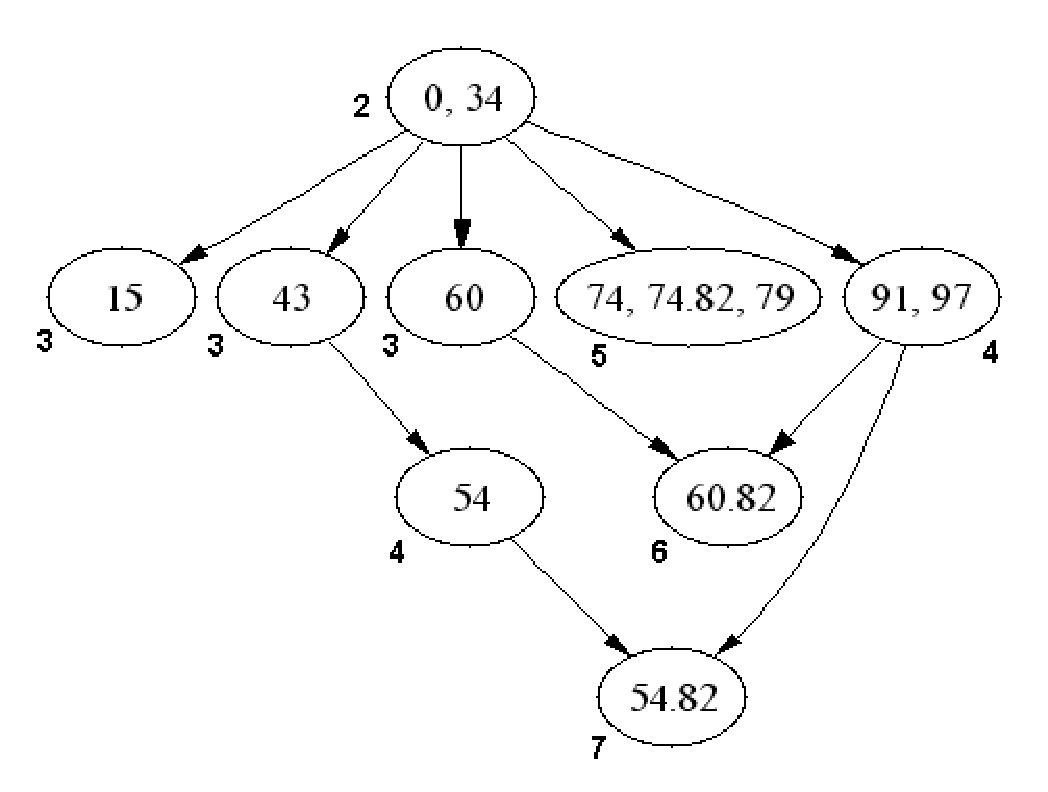
\includegraphics[scale=0.45]{fig/super-block-uncovered.eps}}\qquad
\subfigure[]{\label{fig-super-block-covered}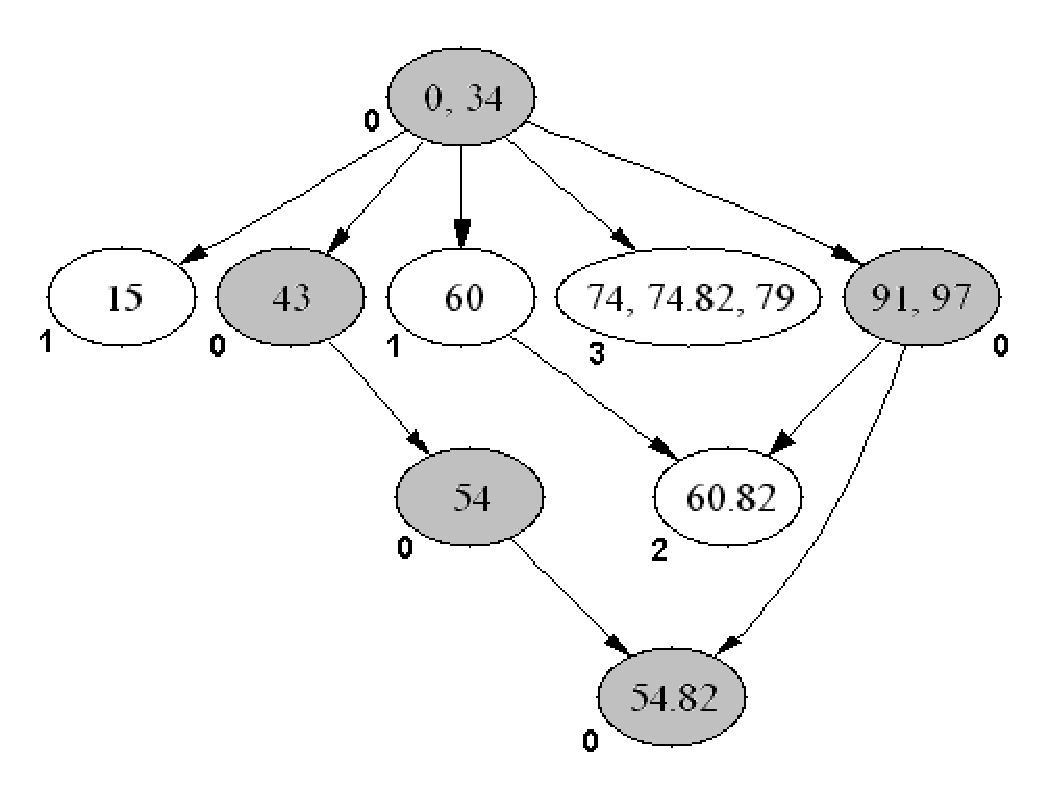
\includegraphics[scale=0.45]{fig/super-block-covered.eps}}
\caption{Super block dominator graph with weights: (a) before any
test case execution, and (b) after the execution of one test
case.}\label{fig-weight}
\end{center}
\end{figure}


Since node 54.82 has a higher weight than node 15, we say that
node 54.82 has a higher priority to be covered than node 15 (\ie,
tests that cover node 54.82 have a higher priority to be executed
than tests that only cover node 15)\footnote{Observe that,
        we are using the term high priority only considering the
        coverage that will be obtained. The tester, based on his
        experience may desire to cover first a node with a lower weight
        but that has a higher complexity in terms of implementation, \ie,
        depending on the criticality of a given part of the code, or based on
        another assumption, the tester can choose to cover a different
        node first and then, by recomputing the weight, to use the weight
        information to increase the coverage faster.
} so that the maximum node coverage can be added in each single
execution. In this way, the node coverage can be increased as much
as possible with as few tests as possible.

After executing certain tests the weights of nodes that are not
covered by these tests may change. For example, after the
execution of a test (say $t_1$) that covers node 54.82 (which also
guarantees the coverage of node 0, 34, 43, 54, 91 and 97), the
execution of another test (say $t_2$) to cover node 15 will
increase the coverage by only one node (namely, node 15 itself).
This is because nodes 0 and 34 have already been covered by test
$t_1$ and the execution of other tests (such as $t_2$) will not
change this fact. Under this scenario, after $t_1$ has been
executed, node 15 will have weight one. This implies that after a
test ($t_1$ in our case) is executed to cover node 54.82, the
priority, in terms of increasing the coverage, of executing
another test ($t_2$ in our case) to cover node 15 may be reduced.

This procedure is applied recursively after the execution of each
test to recompute the weight of each node that has not been
covered by the current tests, as well as the priority of tests to
be executed for covering such nodes. The objective is to continue
this recursive procedure until all the blocks, if possible, are
covered by at least one test (\ie, achieve 100\% node coverage) or
the execution will stop after a predefined time-out been reached.
In the latter case, although tests so executed might not give
100\% node coverage, they still provide as high a block coverage
as possible. \rev{In the reality, as mentioned
in~\cite{Agrawal94DSBP}, the tester only needs to create test
cases that covers one node of each leaf node in the super block
dominator graph to cover all the other nodes.}

\subsection{Program Slicing}\label{sec:slicing}

Computer programmers break apart large programs into smaller
coherent pieces. Each of these pieces: functions, subroutines,
modules, or abstract datatypes, is usually a contiguous piece of
program text. Programmers also routinely break programs into one
kind of coherent piece which is not contiguous. When debugging
unfamiliar programs programmers use program pieces called slices
which are sets of statements related by their flow of control or
data. The statements in a slice are not necessarily textually
contiguous, but may be scattered through a
program~\cite{Weiser82PUSW}. A program slice consists of the parts
of a program that (potentially) affect the values computed at some
point of interest. Such a point of interest is referred to as a
slicing criterion, and is typically specified by a location in the
program in combination with a subset of the program's variables
and/or statements. The task of computing program slices is called
program slicing. The original definition of program slicing was
proposed by Weiser in 1979~\cite{Weiser79PSFP,Weiser84PSLI}.
Today, a lot of slightly different notions of program slices can
be found in the literature, as well as a number of criteria to
compute them~\cite{Tip95SPST}. An important distinction exists
between a static and a dynamic slice. Static slices are computed
without making assumptions regarding a program's input, whereas
the computation of dynamic slices relies on a the execution trace
information of specific test case.

Program slicing is a broadly applicable program analysis technique
that can be used to perform different software engineering
activities, such as: program understanding, debugging, testing,
parallelization, re-engineering, maintenance, and
others~\cite{Gammatech00DGPS}. In the context of \toolname, the
three most important activities are program understanding,
debugging and testing.

\textbf{Program understanding} uses program slicing to help
engineers to understand code. For example, a backward slice from a
point in the program identifies all parts of the code that
contribute to that point. A forward slice identifies all parts of
the code that can be affected by the modification to the code at
the slice point.

\textbf{Testing and Regression Testing} also uses slicing. For
example, suppose a proposed program modification only changes the
value of variable $v$ at program point $p$. If the forward slice
with respect to $v$ and $p$ is disjoint from the coverage of
regression test $t$, then test $t$ does not have to be rerun.
Suppose a coverage tool reveals that a use of variable $v$ at
program point $p$ has not been tested. What input data is required
in order to cover $p$? The answer lies in the backward slice of
$v$ with respect to $p$.

In Section~\ref{sec:slice} it is described the characteristics
\toolname's slicing tool and how to use it to smart debugging and
fault localization.

\subsection{Complexity Metrics}\label{sec:bk-metrics}

Complexity metrics are very useful to several software engineering
tasks. Their main objective is to provide different kinds of
measure of a project/program such that further projects can use
the historical database to better estimate time, cost and
complexity of new projects. There are different kinds of
complexity metrics. For example, Lorenz e Kidd~\cite{Lorenz94OOSM}
defined a set of design metrics to evaluate static characteristics
of an OO software project. The proposed set of metrics is divided
into three groups: 1) \textbf{Class Size Metrics} to quantify
individual classes; 2) \textbf{Class Inheritance Metrics} to
evaluate the quality of using inheritance; and 3) \textbf{Class
Internal Metrics} to evaluate general characteristics of a class.

Another well-known set of metrics, proposer by Chidamber and
Kemerer~\cite{Chidamber94MSOO}, is composed by six design metrics
six design metrics developed to evaluate the complexity of a given
class.

Utsonomia~\cite{Utsonomia02EAMS} have studied and adapted both
sets of design metrics for Java bytecode. \toolname implements
such adapted metrics to allow a tester to collect static metrics
information for the classes under testing.

Another benefit of complexity metrics is that the collected
information can be used to establish incremental testing
strategies by prioritizing the test of certain classes, reducing
the cost and improving the quality of the testing activity. For
instance, \toolname prioritizes testing requirements based on
coverage information. By using complexity metrics, the class's
inheritance, size, and complexity can be combined with coverage
information, providing additional hints to reduce the cost of test
case generation.

In Section~\ref{sec:metrics} it is described how to use \toolname
to collect static information about the classes under testing,
considering the set of complexity metrics adapted from Lorenz e
Kidd~\cite{Lorenz94OOSM} and Chidamber and
Kemerer~\cite{Chidamber94MSOO} works.
